%%%%%%%%%%%%%%%%%%%%%%%%%%%%%%%%%%%%%%%%%%%%%%%%%%%%%%%%%%%%%%%%%%%%%%%%%%%%%%%%%%%%%%%%%%%%%%%%%%%%%%%%%%%%%%%%%%%%%%%%%%%%%%%%%%%%%%%%%%%%%%%%%%%%%%%%%%%%%%%%%%%%%%%
%%%%%%%%%%%%%%%%%%%%%%%%%%%%%%%%%%%%%%%%%%%%%%%%%%%%%%%%%%%%%%%%%%%%%%%%%%%%%%%%%%%%%%%%%%%%%%%%%%%%%%%%%%%%%%%%%%%%%%%%%%%%%%%%%%%%%%%%%%%%%%%%%%%%%%%%%%%%%%%%%%%%%%%
\chapter{Optimisation of the search sensitivity}
\label{sec:Optimisation}
Finally, having all background estimation methods in place, an optimisation procedure is conducted to increase the search sensitivity with respect to the signal models introduced in Section~\ref{sec:SignalSamples}.
The optimisation is done in the most sensitive variables, \pt and \ias.
In this optimisation, the full systematic uncertainty is taken into account, which includes statistical uncertainties arising from limited statistical precision of the samples used in the background estimation methods and the systematic uncertainties that are described in Section~\ref{sec:SysUncertaintiesBkg}.
In order to avoid unnecessary fine-tuning of the optimisation to the specific cross sections of the SUSY models and to keep the search as general as possible, 
the optimisation is not done by maximising  $S/\Delta B$ but by minimising the cross section for which a 5$\sigma$ discovery is possible
\begin{equation}
\label{eq:optimisation}
\frac{\sigma_{\text{min}}\cdot \mathcal{L}}{\Delta B} = \frac{\sigma_{\text{min}}\cdot \mathcal{L}}{\sqrt{ \Delta B_{\text{stat}} + \Delta B_{\text{sys}}}} \geq 5.
\end{equation} 
In this formula, $\mathcal{L}$ is the integrated luminosity in 2012, $\sigma_{\text{min}}$ is the cross section to be minimised, $\Delta B_{\text{sys}}$ is the systematic uncertainty of the background prediction as explained above and 
$\Delta B_{\text{stat}}$ is the statistical uncertainty of the background prediction which is the 68\% one sided upper limit of a poisson distribution with $\mu = B$ estimated with the 
Neyman construction~\cite{bib:Neyman_1937,bib:PDG_2014}.

Four different benchmark models are choosen for the optimisation.
As this analysis focus on short tracks, models with charginos with low lifetimes are choosen: $\ctau=1\cm$ and $\ctau=5\cm$. 
Additionally, two different masses in order to cover also the mass dimension: 100\gev and 500\gev.

A visualised optimisation is done by imposing general systematic uncertainties on the leptonic and the fake background of 100\% and 20\% respectively whereas
the uncertainties arising from limited statistical precision of the samples are propagated accurately into the formula~\ref{eq:optimisation}.
The results can be found in Fig.~\ref{fig:optimisation}, where the minimal cross section that is possible to exclude is shown in the $\pt-\ias$ plane.
\begin{figure}[!h]
  \centering 
  \begin{tabular}{c}
    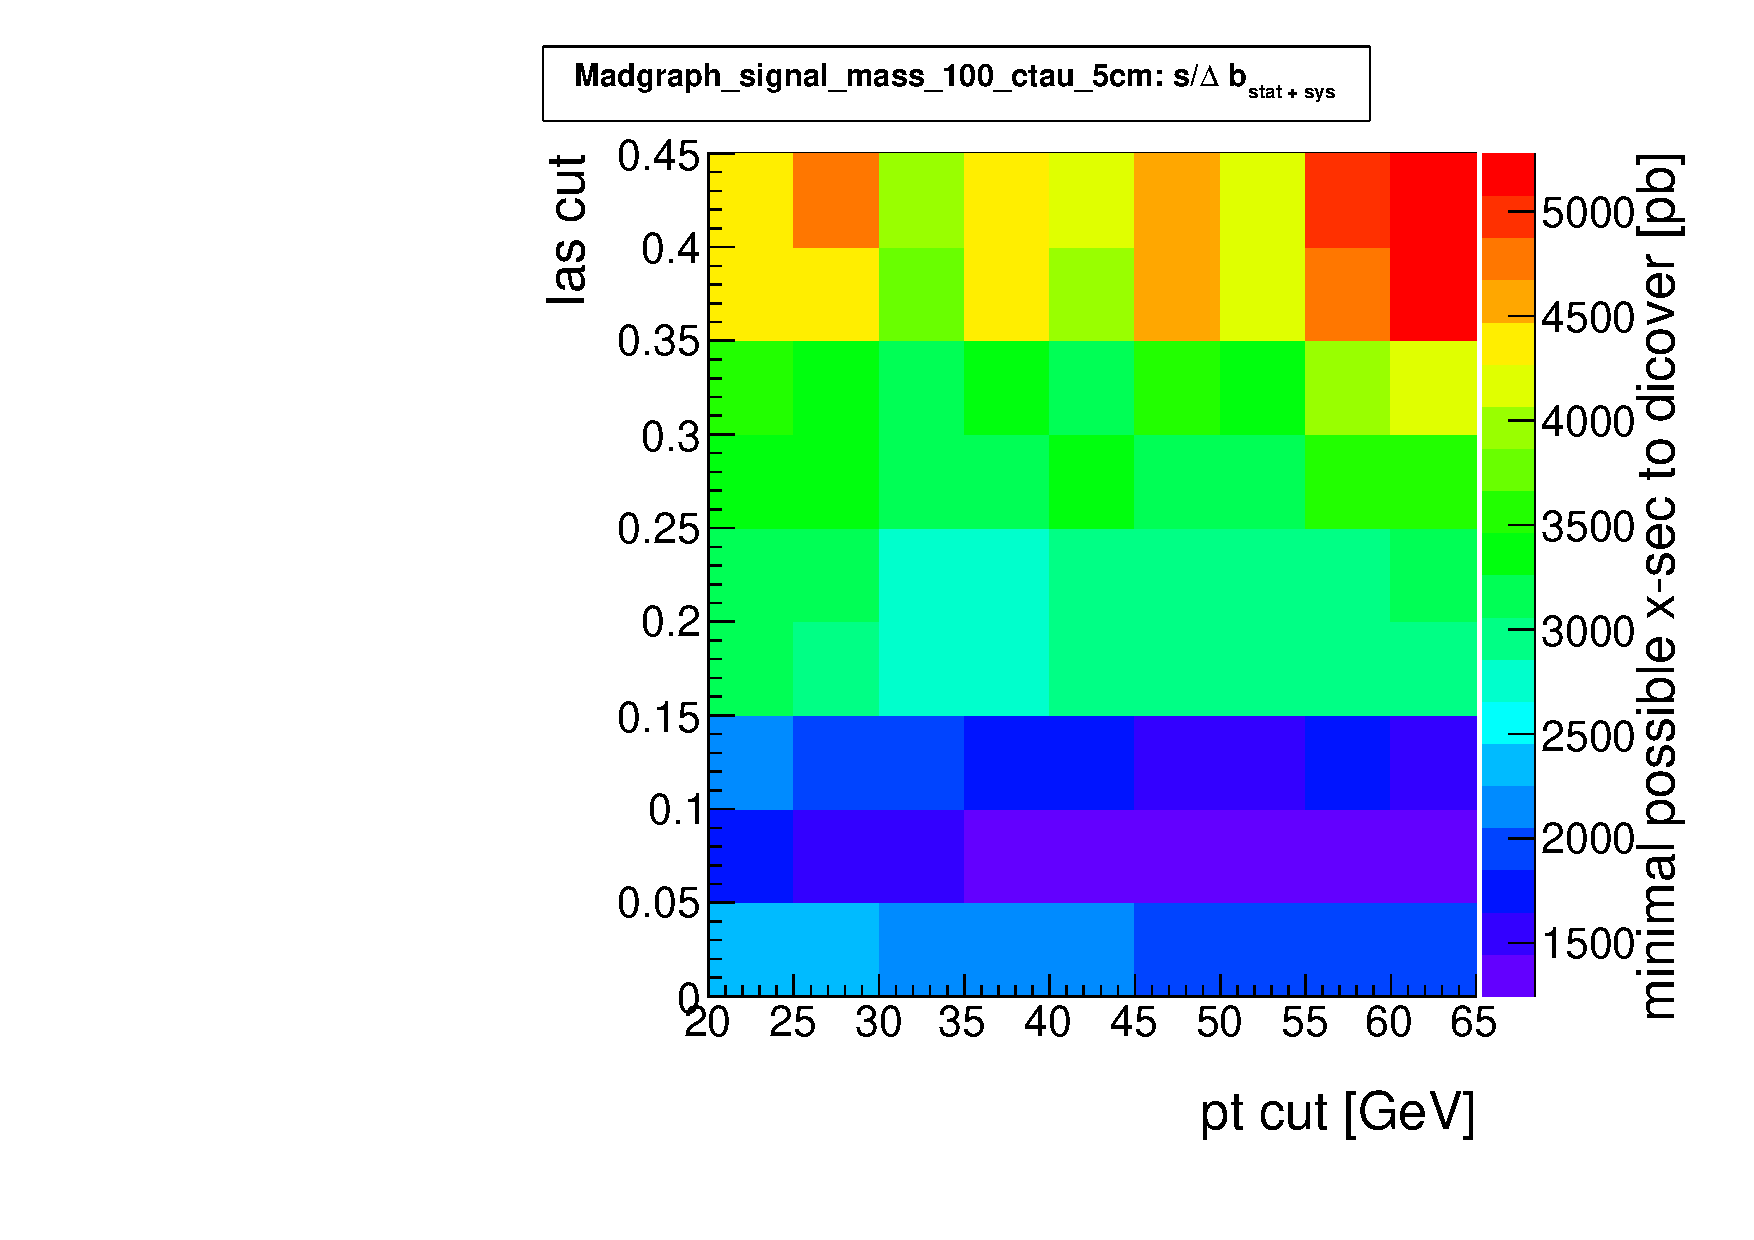
\includegraphics[width=0.49\textwidth]{figures/analysis/Optimisation/Madgraph_signal_mass_100_ctau_5cm_ECaloLe5_SOverDeltaBStatPlusSys.pdf} 
    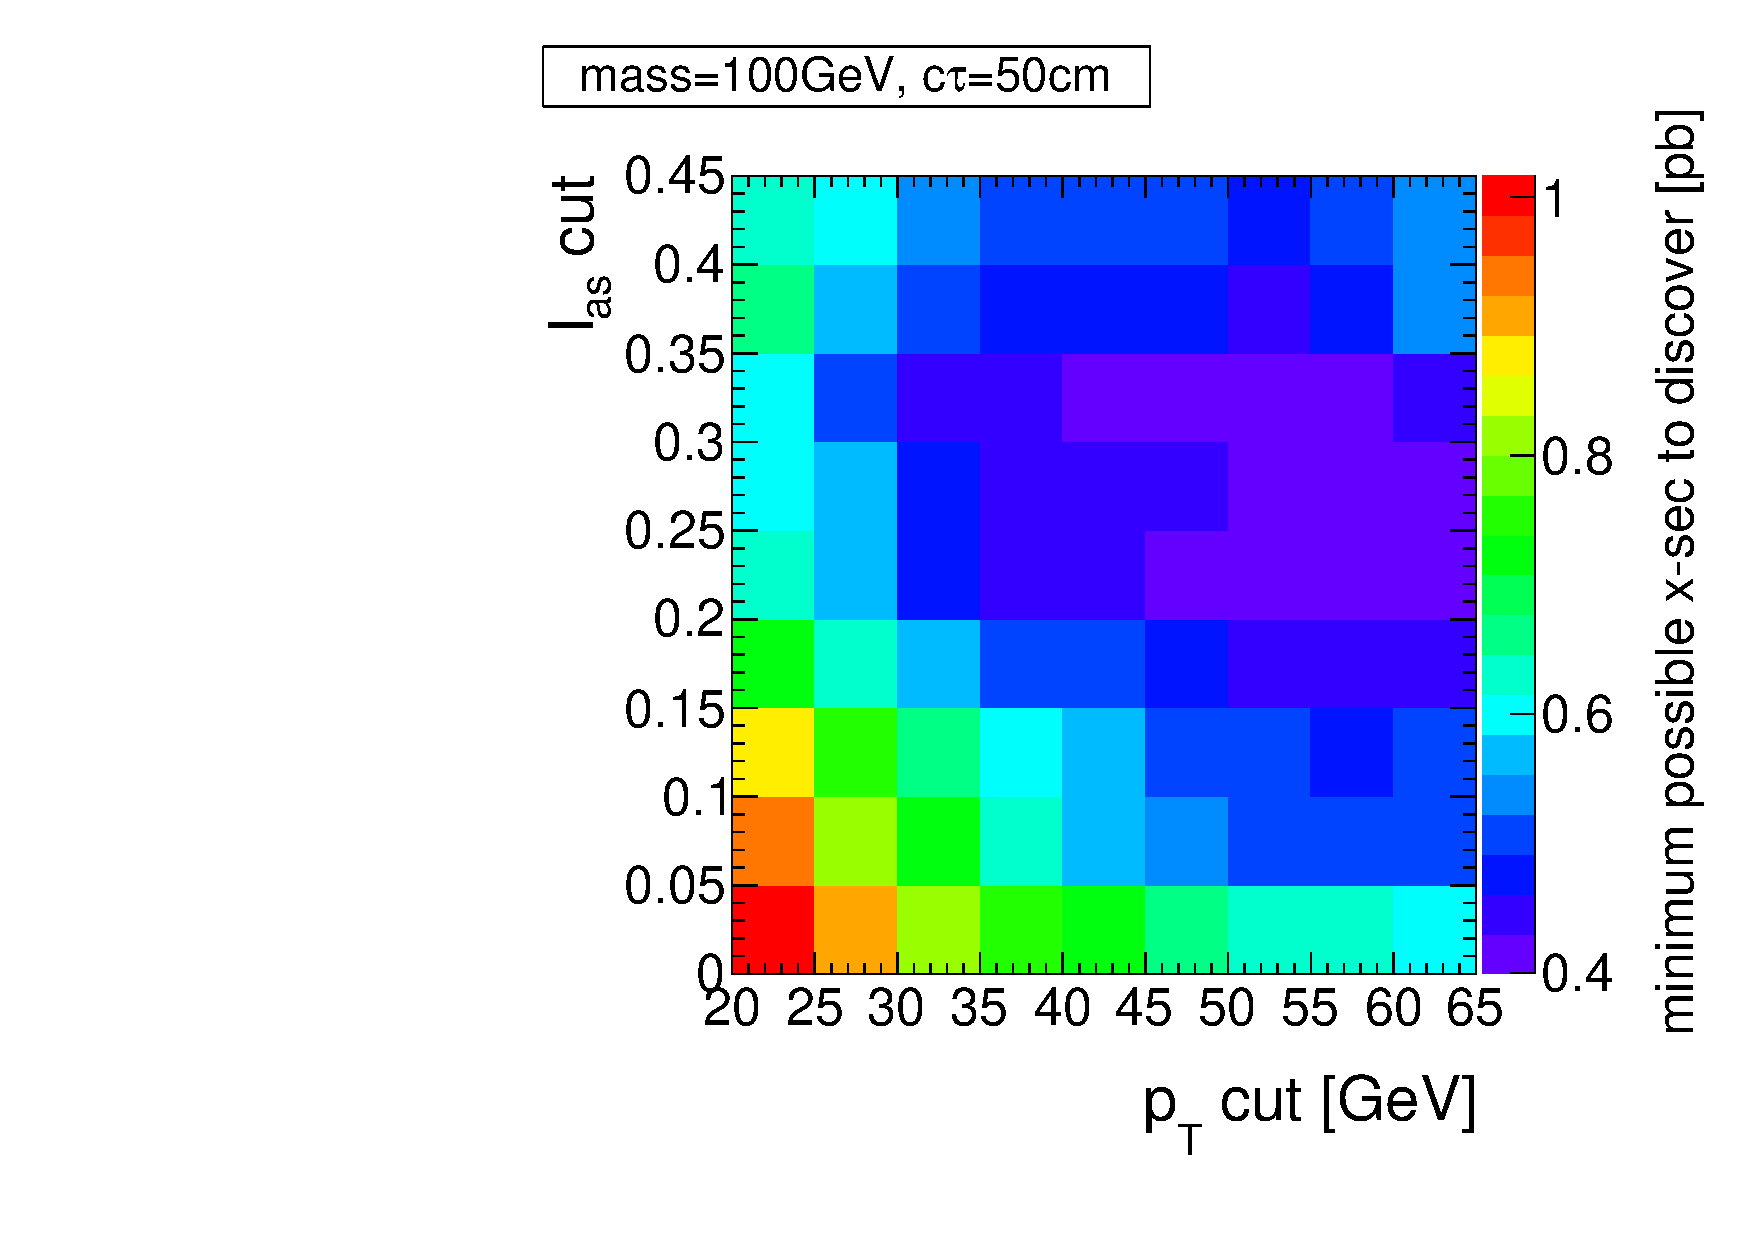
\includegraphics[width=0.49\textwidth]{figures/analysis/Optimisation/Madgraph_signal_mass_100_ctau_50cm_ECaloLe5_SOverDeltaBStatPlusSys.pdf}\\ 
    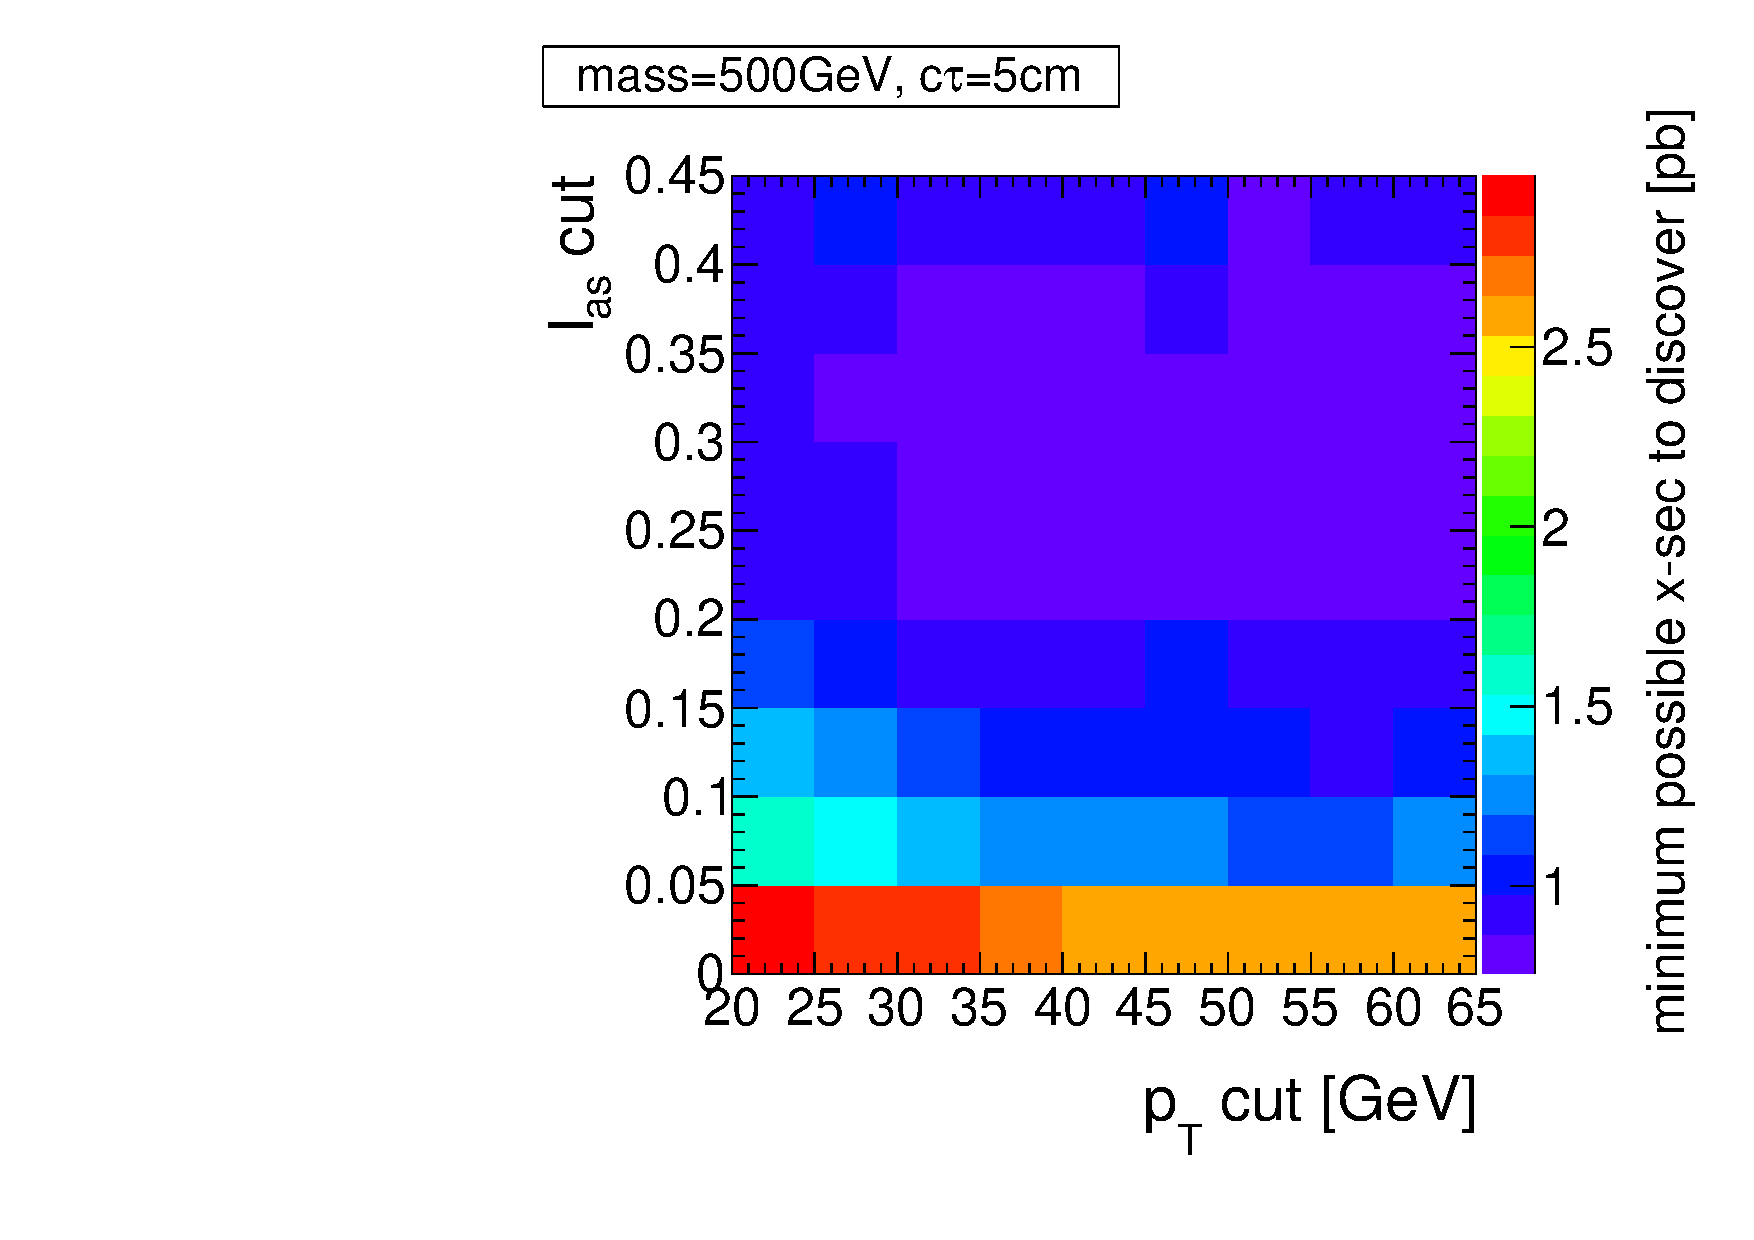
\includegraphics[width=0.49\textwidth]{figures/analysis/Optimisation/Madgraph_signal_mass_500_ctau_5cm_ECaloLe5_SOverDeltaBStatPlusSys.pdf}
    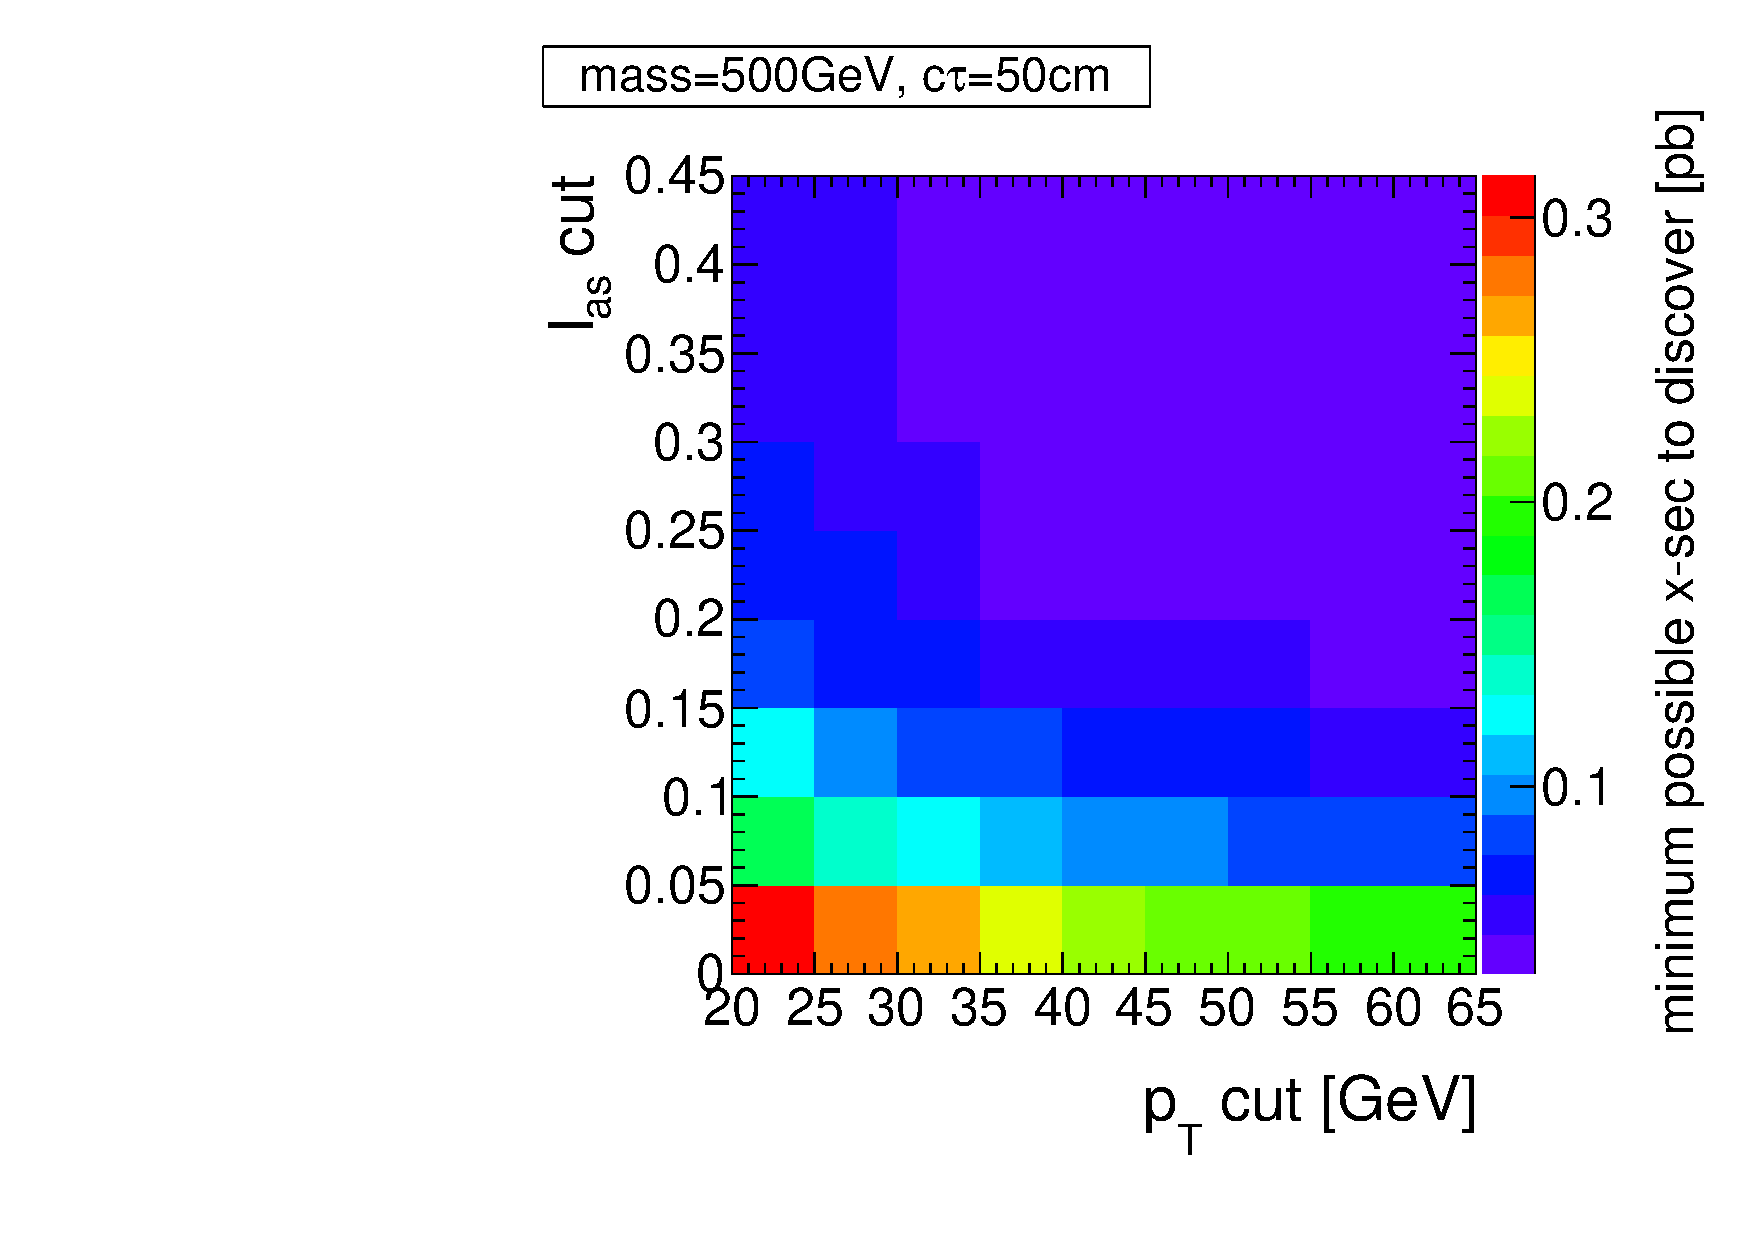
\includegraphics[width=0.49\textwidth]{figures/analysis/Optimisation/Madgraph_signal_mass_500_ctau_50cm_ECaloLe5_SOverDeltaBStatPlusSys.pdf} 
  \end{tabular}
  \caption{Minimal possible cross section to exclude in the $\ias-\pt$ plane for four different signal models.}
  \label{fig:optimisation}
\end{figure} 
A exact optimisation taken the whole background uncertainties precisly into account is done without a visualisation.
The corresponding results are shown in Table~\ref{tab:optimisation}.

\renewcommand{\arraystretch}{1.5}
\begin{table}[!h]
\centering
\caption{Optimal \pt and \ias cuts and corresponding minimal possible cross section $\sigma_{\text{min}}$ to exclude for different signal models.}
\label{tab:optimisation}
\makebox[0.99\textwidth]{
\begin{tabular}{c |c| c| c| c}
\multicolumn{5}{c}{} \\
\toprule
Mass [\gev] & Lifetime [\cm] & Optimal \pt cut & Optimal \ias cut & $\sigma_{\text{min}}$ \\
\midrule
100&                           1&                             30&                            0.05&                          59.0291   \\
500&                           1&                             0 &                            0.0 &                          10000.0000\\
100&                           5&                             50&                            0.05&                          2.6965    \\
500&                           5&                             50&                            0.30&                          0.6180    \\
\bottomrule
\multicolumn{5}{c}{} \\
\end{tabular}}
\end{table}

It can be seen that the optimal selections are highly dependent on the signal models.

Additionally, it is checked whether a sensitivity increase can be achieved by imposing also a selection on the number of missing outer hits $N_{lost}^{outer}$.
For low lifetimes, a tiny increase in sensistivy is possible by selecting also in this variable but as this variable comes with new sources of uncertainties this is not consideres in this search.

To have an optimal coverage over a wide mass space, four different signal regions are defined:
\begin{enumerate}
\item $30\gev<\pt<50\gev$ and $0.05<\ias<0.3$
\item $30\gev<\pt<50\gev$ and $\ias>0.3$
\item $\pt>50\gev$ and $0.05<\ias<0.3$
\item $\pt>50\gev$ and $\ias>0.3$.
\end{enumerate}

%%%%%%%%%%%%%%%%%%%%%%%%%%%%%%%%%%%%%%%%%%%%%%%%%%%%%%%%%%%%%%%%%%%%%%%%%%%%%%%%%%%%%%%%%%%%%%%%%%%%%%%%%%%%%%%%%%%%%%%%%%%%%%%%%%%%%%%%%%%%%%%%%%%%%%%%%%%%%%%%%%%%%%%
%%%%%%%%%%%%%%%%%%%%%%%%%%%%%%%%%%%%%%%%%%%%%%%%%%%%%%%%%%%%%%%%%%%%%%%%%%%%%%%%%%%%%%%%%%%%%%%%%%%%%%%%%%%%%%%%%%%%%%%%%%%%%%%%%%%%%%%%%%%%%%%%%%%%%%%%%%%%%%%%%%%%%%%
\chapter{Results}
\label{sec:Results}

After the development of the background estimation methods for all different background sources and their corresponding systematic uncertainties (all explained in Section~\ref{sec:BackgroundEstimation}), 
the search is performed in four different signal regions with 19.7\fbinv of data collected at a centre-of-mass energy of $\sqrt{s} = 8\tev$ at the CMS experiment.
The comparison between the predicted number of events and the number of observed events is shown in Fig.~\ref{fig:FinalResult}.
\begin{figure}[!b]
  \centering 
  \begin{tabular}{c}
    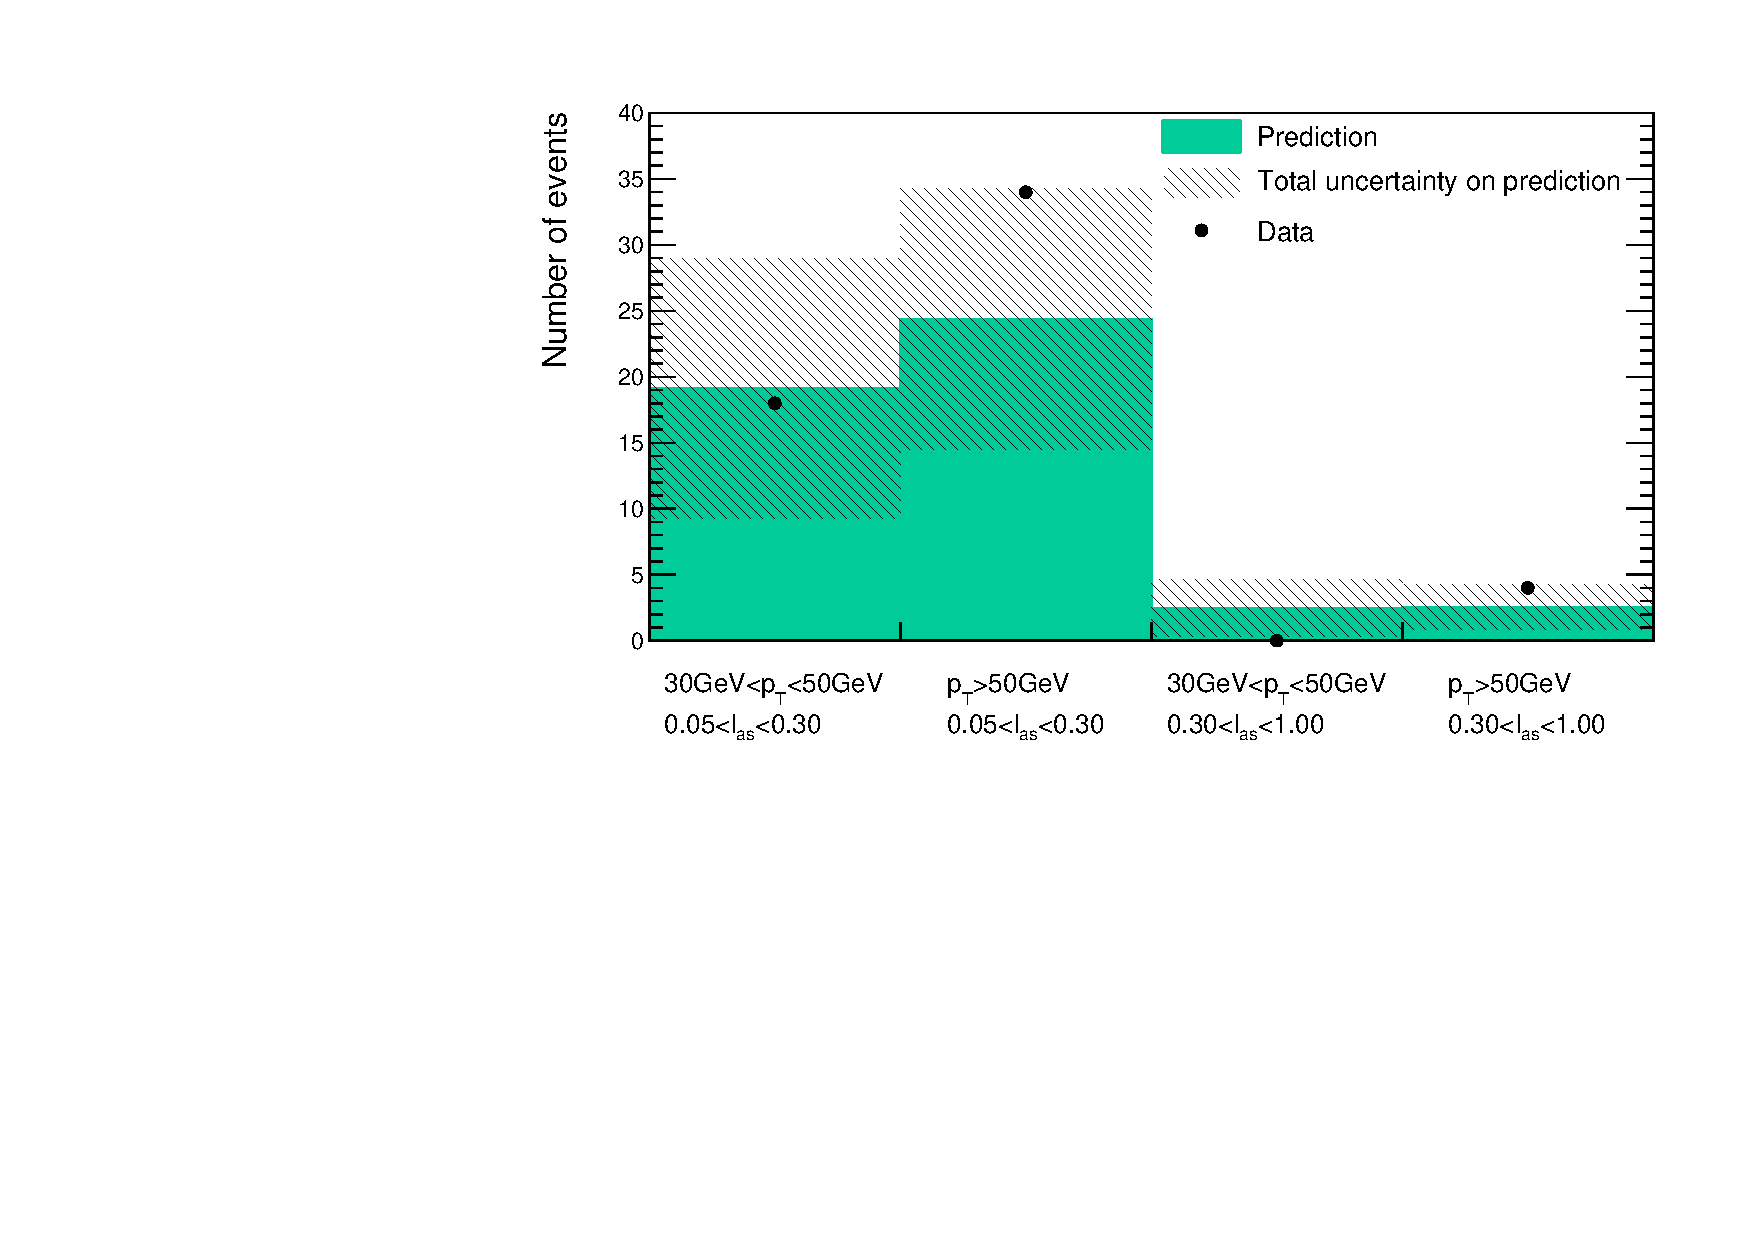
\includegraphics[width=0.99\textwidth]{figures/analysis/Results/FinalResultPlot.pdf} 
  \end{tabular}
  \caption{Number of predicted (green area) and observed (black dots) events for the four different signal regions. The hashed area represents the total uncertainty on the background prediction.}
  \label{fig:FinalResult}
\end{figure} 
The corresponding numbers of predicted and observed events can be found in Table~\ref{tab:FinalResult}.
\renewcommand{\arraystretch}{1.5}
\begin{table}[!h]
\centering
\caption{Number of predicted and observed events for the four different signal regions.}
\label{tab:FinalResult}
\makebox[0.99\textwidth]{
\begin{tabular}{l |c| c}
\multicolumn{3}{c}{} \\
\toprule
Signal region                           & Prediction & Observation  \\
\midrule
$30\gev<\pt<50\gev$ and $0.05<\ias<0.3$ & 0          &0 \\
$30\gev<\pt<50\gev$ and $\ias>0.3$      & 0          &0 \\
$\pt>50\gev$ and $0.05<\ias<0.3$        & 0          &0 \\
 $\pt>50\gev$ and $\ias>0.3$       & 0          &0 \\
\bottomrule
\multicolumn{3}{c}{} \\
\end{tabular}}
\end{table}
The event yields observed in data after each selection requirement for the four signal regions are listed in Table~\ref{FIXME} in Appendix~\ref{FIXME}.

The results are compatible in all four signal regions with the Standard Model background within the 1$\sigma$ uncertainties.
No excess above the SM prediction is in either of the four signal regions observed.
That means, there is no evidence for physics beyond the Standard Model.

Therefore, in the following section the result is interpreted within the context of a supersymmetric model with a wino-like \chipm and \chiO.

%%%%%%%%%%%%%%%%%%%%%%%%%%%%%%%%%%%%%%%%%%%%%%%%%%%%%%%%%%%%%%%%%%%%%%%%%%%%%%%%%%%%%%%%%%%%%%%%%%%%%%%%%%%%%%%%%%%%%%%%%%%%%%%%%%%%%%%%%%%%%%%%%%%%%%%%%%%%%%%%%%%%%%%
%%%%%%%%%%%%%%%%%%%%%%%%%%%%%%%%%%%%%%%%%%%%%%%%%%%%%%%%%%%%%%%%%%%%%%%%%%%%%%%%%%%%%%%%%%%%%%%%%%%%%%%%%%%%%%%%%%%%%%%%%%%%%%%%%%%%%%%%%%%%%%%%%%%%%%%%%%%%%%%%%%%%%%%
\chapter{Interpretation}
\label{sec:Interpretation}
In order to interpret the result of the search in the context of supersymmetric models with wino-like \chipm and \chiO, the size of uncertainties of the simulated signal events must be estimated.
Furthermore, the size of correlations between the systematic uncertainties must be determined to be able to combine the results of all four signal regions.
The interpretation will then be done with statistical methods, that allow for exclusions of parts of the supersymmetric parameter space on a 95\% confidence level.

\section{Systematic uncertainties of simulated signal samples}
The systematic uncertainties on the number of signal events in the four signal regions are mainly caused by uncertainties on the quality of the simulation.
This influences the signal efficiency of every selection requirements done in this analysis.
Furthermore, an uncertainty on the overall number of events is caused by the uncertainty on the integrated luminosity recorded in 2012 at CMS and the theoretical signal cross-sections.

\subsection*{Luminosity uncertainty}
The integrated luminosity recorded at CMS during the year 2012 is not exactly known. 
A detailed explanation of the methods to measure the luminosity and the corresponding total uncertainty of 2.6\% can be found in \cite{bib:CMS:Lumi_PAS}.

\subsection*{Uncertainty on the simulation of initial state radiation}
This uncertainty is estimated via a comparison of simulated and observed $Z$ and $\bar{t}t$ events done in~\cite{bib:CMS:ISR_AN}.
In order to take data-simulation differences of initial state radiation into account, the transverse momentum of the $\chipm\chimp$ or $\chipm\chiO$ system is reweighted.
The uncertainty of the reweighted procedure is taken into account as changes of the weight up to 25\%.

\subsection*{Uncertainty on the simulation of the trigger efficiency}
The HLTMonoCentralPFJet80\_PFMETnoMu105\_NHEF0p95 trigger used in this analysis was not available in the simulated signal samples.
It was therefore emulated using L1 information. More details on the emulation of this trigger can be found in Appendix~\ref{FIXME}.

The trigger uncertainty is accessed by comparing data-simulation differences of the trigger efficiency.
This has been done within~\ref{bib:CMS:DT_Thesis,bib:CMS:DT_8TeV_AN}.
The resulting differences are applied as variations in event weights on the simulated samples.
The corresponding uncertainty lies between $2.6-4.6\%$ for the signal samples.

\subsection*{Uncertainty on the jet energy scale}
The uncertainty on the jet energy scale arise from various unknows, neatly described in~\cite{bib:CMS:JME_PAS}.
The correction applied as a multiplicant on each jet's transverse momentum conatined in an event is varied up and down within 1sigma.
The resulting uncertainties are of minor importance and lie between $0.5-1.1\%$.

\subsection*{Uncertainty on the jet energy resolution}
The jet energy resolution is smaller in simulated than in measured data.
To take into account these differences, the jet energy response is additionnaly smeared to match the measured response.
The corresponding uncertainties are estimated in order to cover the uncertainty on the measured resolution in data.
The resulting uncertainty on the signal efficiency is between $0.1-0.7\%$ and therefore almost negliglbe . CITE SOMETHING

\subsection*{Uncertainty on the simulation of the parton density functions}
The uncertainty on the simulation of the parton density function is a complex procedure, very well described in CITEME.
The resulting uncertainties are within blabla.

\subsection*{Uncertainty on the simulation of the calorimeter isolation}
\subsection*{Uncertainty on the simualtion of missing middle hits}
\subsection*{Uncertainty on the simulation of missing inner hits}
\subsection*{Uncertainty on the simulation of pile-up}
\subsection*{Uncertainty on the simulation of the track reconstruction efficiency}
\subsection*{Uncertainty on the simulation of the \ias}
\subsection*{Uncertainty on the theoretical cross section}

%%%%%%%%%%%%%%%%%%%%%%%%%%%%%%%%%%%%%%%%%%%%%%%%%%%%%%%%%%%%%%%%%%%%%%%%%%%%%%%%%%%%%%%%%%%%%%%%%%%%%%%%%%%%%%%%%%%%%%%%%%%%%%%%%%%%%%%%%%%%%%%%%%%%%%%%%%%%%%%%%%%%%%%
\section{Correlation of systematic uncertainties}
In order to combine the four different signal regions, a specification of the size of correlations between the systematic uncertay needs to be addresses.

\subsection*{Background correlations}
\subsection*{Signal correlation}
%%%%%%%%%%%%%%%%%%%%%%%%%%%%%%%%%%%%%%%%%%%%%%%%%%%%%%%%%%%%%%%%%%%%%%%%%%%%%%%%%%%%%%%%%%%%%%%%%%%%%%%%%%%%%%%%%%%%%%%%%%%%%%%%%%%%%%%%%%%%%%%%%%%%%%%%%%%%%%%%%%%%%%%
\section{Statistical Methods/ Limit setting}

Finally, bla bla bla.
%%%%%%%%%%%%%%%%%%%%%%%%%%%%%%%%%%%%%%%%%%%%%%%%%%%%%%%%%%%%%%%%%%%%%%%%%%%%%%%%%%%%%%%%%%%%%%%%%%%%%%%%%%%%%%%%%%%%%%%%%%%%%%%%%%%%%%%%%%%%%%%%%%%%%%%%%%%%%%%%%%%%%%%
\section{Exclusion limits}
\begin{itemize}
\item 1-d limits
\item 2-d limits
\end{itemize}


%%%%%%%%%%%%%%%%%%%%%%%%%%%%%%%%%%%%%%%%%%%%%%%%%%%%%%%%%%%%%%%%%%%%%%%%%%%%%%%%%%%%%%%%%%%%%%%%%%%%%%%%%%%%%%%%%%%%%%%%%%%%%%%%%%%%%%%%%%%%%%%%%%%%%%%%%%%%%%%%%%%%%%%
\chapter{Discussion and outlook and conclusion}
\label{sec:Discussion}
